% Chapitre 12 -- N2 : le réseau triangulaire n'est pas un minimum local de l'énergie de point zéro pour Yukawa kappa = 1, 2
% Sources : results/discovery_journal_2026/TOP20.json (pick 12), papers/p3_zero_point_physical/{main.tex,AUDIT.md,REVISION.md,publication_meta.json,data/}.
% Figure : code/spare_fig12.py.
\chapter[Le meilleur n'est pas le plus calme]{Le meilleur rangement n'est pas le plus calme}

\reference{Publié le 26 octobre 2026. doi:10.5281/zenodo.23663551}

\section*{L'idée en une image}

Le travail précédent, sur la répulsion en cloche, concernait une force commode pour les
mathématiciens. Ce chapitre reprend la même question pour une force que l'on rencontre vraiment : la
répulsion entre charges électriques \og écrantée\fg{} par leur entourage, comme dans un plasma
ou entre des grains en suspension. On l'appelle force de Yukawa ; elle vaut $e^{-\kappa r}/r$ à
la distance $r$, et le nombre $\kappa$ dit à quelle vitesse l'écran l'éteint. On a étudié
$\kappa=1$ et $\kappa=2$, pour des particules posées dans un plan.

Pour cette force, un travail antérieur du projet, sur la force de Yukawa au repos, établit que le réseau triangulaire
est le meilleur arrangement régulier \emph{au repos}, sous réserve d'un théorème amont produit
par une IA et pas encore relu par des pairs. La question devient : ce champion du repos est-il
aussi le plus économe quand on compte le frisson quantique de point zéro ?

\begin{analogie}
Des billes qui se repoussent sur un plateau, en nombre fixé par mètre carré. Immobiles, elles
choisissent les triangles. Mais faites-les trembler : on découvre qu'en penchant très légèrement
le motif, le tremblement coûte un peu moins cher. Le meilleur rangement n'est pas le plus calme.
\emph{Où l'image s'arrête :} le tremblement dont il s'agit n'est pas celui de la chaleur, c'est
le frisson quantique qui subsiste au zéro absolu ; et l'on ne compare que ce frisson, pas
l'énergie totale du cristal.
\end{analogie}

\section*{Ce qui a été fait}

La première idée était de réutiliser le \og toit\fg{} du travail sur la cloche : une fonction
au-dessus de l'énergie, qui la touche au départ. Pour la force de Yukawa, ce toit ne sert à
rien : sa courbure certifiée est \emph{positive} (entre $2{,}393$ et $2{,}464$ pour $\kappa=1$),
alors que la vraie courbure, calculée de façon approchée, est négative. Le toit est trop haut ;
il ne peut rien dire du terrain.

D'où la nouveauté du papier : un toit qui \emph{suit} le terrain. Au lieu d'une estimation
fixe, on utilise une estimation qui bouge avec la déformation, au premier ordre. Ce nouveau toit
reste au-dessus de l'énergie, la touche au départ, et a exactement la même courbure qu'elle en
ce point. Le calcul certifié borne alors sa courbure par $-2{,}03704$ ($\kappa=1$) et
$-1{,}86854$ ($\kappa=2$) sur toute la fenêtre $|t|\le10^{-5}$ : le réseau triangulaire n'est
pas un minimum local de l'énergie de point zéro.

\begin{encadre}
\textbf{À faire avec un crayon : pourquoi un toit fixe est trop haut.} Suivons $\sqrt{d}$ quand
$d(t)=(2+t)^2$ ; la vraie racine vaut $2+t$, une droite, de courbure nulle.
\emph{Toit fixe} (estimation $x=2$) :
$\tfrac12\bigl(2+\tfrac{d}{2}\bigr)=2+t+\tfrac{t^2}{4}$, de courbure $\tfrac12>0$ : il reste
au-dessus, mais il se courbe vers le haut alors que la vraie courbe ne se courbe pas.
\emph{Toit mobile} (estimation $x=2+t$) : $\tfrac12\bigl((2+t)+\tfrac{(2+t)^2}{2+t}\bigr)=2+t$,
exactement la vraie courbe. Le papier fait la même chose avec des matrices $2\times2$, et
l'estimation mobile n'y est exacte qu'au premier ordre, ce qui suffit pour la courbure.
\end{encadre}

Le préenregistrement listait six forces. Deux sont certifiées. Pour trois autres (une force en
$1/r^3$ et deux forces de dipôles), le certificat bute sur la queue des sommes : la borne du
reste décroît trop lentement, en $6800/R$ environ pour un rayon de coupure $R$, contre une marge
de $3{,}8$ ; il faudrait $R$ de l'ordre de $10^5$, hors de portée. Une parade est esquissée, non
tentée, et rien n'est affirmé pour ces forces. La sixième ($1/r^4$) n'a pas été tentée : le calcul
approché suggère qu'il s'agit d'un minimum local, et la question annoncée confondait sans doute
\og pas le meilleur partout\fg{} et \og pas le meilleur tout près\fg{}.

\section*{Comment on s'est assuré que ce n'est pas faux}

Le résultat d'ensemble est \niveau{C}, comme pour la cloche : la logique et le signe des
fractions sont \niveau{A} \emph{Le juge a regardé} (vérifiés par le noyau de Lean, axiomes dans la liste courte, et un
rejeu par le noyau des trois modules concernés est passé), les intégrales sont encadrées par une
arithmétique d'intervalles rigoureuse (86\,581 cellules, aucune en échec) exécutée par un
programme, et la colle est un raisonnement mené par des agents d'IA, que personne n'a vérifié à la machine.

Les contrôles : la cloche $e^{-\pi r^2}$ redonne bien \og pas un minimum\fg{} ; la cloche
$e^{-2\pi r^2}$, où le réseau triangulaire est un minimum, n'est pas certifiée (sa courbure est
encadrée entre $+3{,}45$ et $+4{,}46$), comme il le faut ; un premier essai trop grossier pour
$\kappa=1$ n'a rien certifié et il est conservé dans les données. Un agent auditeur distinct a
relu le code, refait les dérivations à la main et relancé deux calculs, qui ont redonné les mêmes
nombres au bit près. Verdict : \og accepter avec corrections\fg{}, sans point bloquant ; douze
corrections, surtout des phrases trop fortes, ont été appliquées. Aucun humain n'a relu ce
travail, et l'énoncé Lean n'est pas verrouillé.

\section*{Ce que ça ne dit pas}

\begin{limite}
\begin{itemize}
\item Deux forces sur six ; une fenêtre de $10^{-5}$ ; un seul chemin de déformation ; deux
  dimensions ; réseaux réguliers ; approximation harmonique.
\item Rien sur l'énergie totale : au repos, la courbure est positive, si bien que pour un vrai
  cristal à faible frisson rien ne suit, et aucune transition de structure n'est annoncée.
\item \og Champion au repos\fg{} repose sur le travail sur Yukawa au repos, lui-même conditionnel à un théorème
  produit par une IA.
\item Les forces en $1/r^3$ et les dipôles restent ouverts, dans un sens comme dans l'autre.
\end{itemize}
\end{limite}

La leçon tient en une phrase : optimal au repos ne veut pas dire optimal en frissonnant, et pour
la première fois le projet le sait avec un certificat, pour des forces physiques.

\section*{Pour aller plus loin}

Le papier (10 pages, en anglais), avec le tableau des six forces et l'obstacle détaillé :
doi:10.5281/zenodo.23663551.\par Travaux liés : la cloche,\\ doi:10.5281/zenodo.23655392 ;\\ Yukawa au repos,\\ doi:10.5281/zenodo.23646105.

\begin{figure}[ht]
\centering
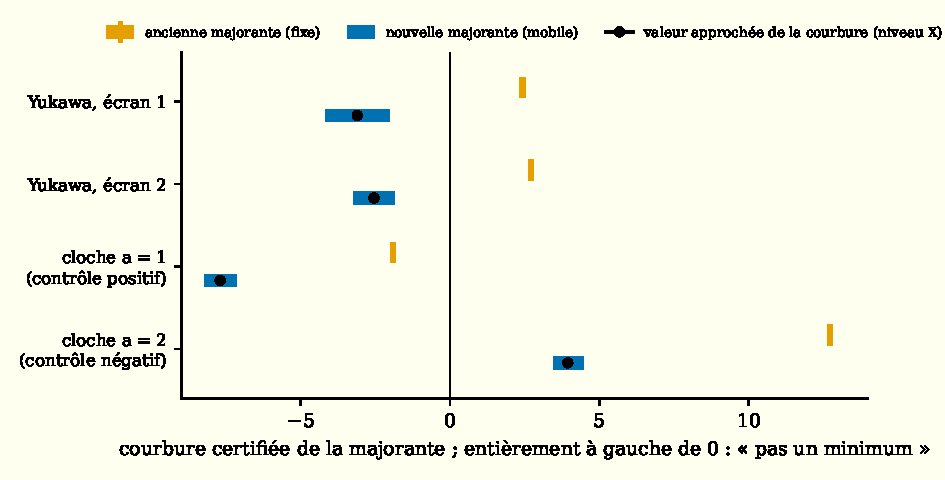
\includegraphics[width=\linewidth]{figures/spare_c12_majorantes}
\caption{Courbures certifiées : l'ancien toit (orange) est positif pour Yukawa, le nouveau (bleu) négatif ; le contrôle $a=2$ reste positif.}
\end{figure}
